\subsubsection{Metode SMOTE}

Metode \textit{Synthetic Minority Over-sampling Technique} (SMOTE) \cite{chawla2002smote} menggunakan pendekatan \textit{over-sampling} yang mana kelas minoritas ditambah dengan membuat sampel "sintetis" bukan dengan mengganti sampel dari kelas mayoritas menjadi kelas minoritas.
Sampel sintetis dibuat lebih kurang lewat aplikasi, dengan beroperasi pada "ruang fitur" bukan pada "ruang data".
Kelas minoritas ditambah dengan mengambil setiap sampel-sampel dari kelas minoritas dan membuat sampel sintetis diantara segmen garis yang menggabungkan setiap/semua \textit{k-nearest-neighbors} dari kelas minoritas.
Bergantung kepada jumlah \textit{over-sampling} yang dibutuhkan, instan dari \textit{k-nearest-neighbors} dipilih secara acak.

\begin{figure}[t]
	\centering
	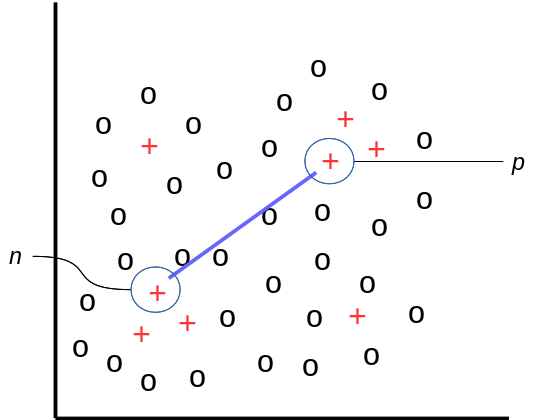
\includegraphics[keepaspectratio=true,scale=0.6]{SMOTE-example}
	\caption{Ilustrasi pembuatan sampel sintetis pada SMOTE.
		\textit{p} adalah sampel minoritas, \textit{n} adalah salah satu \textit{k-nearest-neighbors} dari \textit{p}.
		Sampel sintetis yang baru akan berada digaris antara \textit{p} dan \textit{n}.
	}
	\label{fig:smote}
\end{figure}

Sampel sintetis dibuat dengan cara berikut,
\begin{itemize}
	\item Hitung selisih antara vektor fitur (sampel) dengan tetangga terdekatnya.
	\item Kalikan selisih tersebut dengan angka ril acak antara 0 sampai 1, dan
	\item tambahkan hasilnya ke vektor fitur.
\end{itemize}

Cara ini membuat sampel secara acak pada segmen garis antara dua fitur yang terpilih, seperti yang terlihat pada gambar \ref{fig:smote}.
Pendekatan ini secara efektif mendorong wilayah pembelajaran dari kelas minoritas menjadi lebih besar tanpa menyebabkan \textit{overfitting}.

Ambil contoh sebuah sampel (6,4) dan (4,3) sebagai tetangga terdekatnya.
(6,4) adalah sampel yang akan dicari \textit{k-nearest-neighbors}-nya.
(4,3) adalah salah satu dari \textit{k-nearest-neighbors}-nya.
Misalkan,
\[
\begin{matrix}
f1\_1 = 6 & f1\_2 = 4 \\
f2\_1 = 4 & f2\_2 = 3
\end{matrix}
\]
\[
\begin{matrix}
f2\_1 - f1\_1 = 4 - 6 = -2 \\
f2\_2 - f1\_2 = 3 - 4 = -1
\end{matrix}
\]

Sampel baru dihasilkan dengan,
\[
(f1', f2') = (6,4) + random(0-1) * (-2,-1)
\]

Fungsi \texttt{random(0-1)} menghasilkan bilangan ril acak dari 0 sampai 1.


\subsubsection{Metode LN-SMOTE}

Meskipun hasil SMOTE dibuktikan bagus dalam makalah Chawla dkk. \cite{chawla2002smote}, metode ini masih memiliki beberapa kelemahan.
Pertama, cara menentukan sampel minoritas sebagai calon untuk \textit{over-sampling} bisa bermasalah.
Dalam metode SMOTE semua sampel dari kelas minoritas digunakan.
Namun, bukan berarti semua sampel tersebut sama bergunanya bagi pembelajaran klasifikasi.
Pada khususnya, sampel yang ada pada batas \textit{decision}, atau berada dibatas kelas minoritas dengan kelas mayoritas, lebih sering salah diklasifikasi dibandingkan dengan sampel yang berada jauh dari batas kelas, oleh karena itu mereka lebih penting untuk klasifikasi.
Sampel yang jauh dari batas kelas, berada di tengah kelas minoritas mungkin berkontribusi sedikit pada klasifikasi.
Salah satu metode untuk menangani permasalahan ini yaitu dengan hanya mengambil sampel pada batas kelas minoritas yang dijadikan untuk \textit{oversampling}, seperti yang diajukan oleh Han dkk. \cite{han2005borderline} dengan menggunakan metode bernama \textit{Borderline SMOTE}.

\begin{figure}[b!]
	\centering
	\begin{subfigure}[b]{0.4\textwidth}
		\centering
		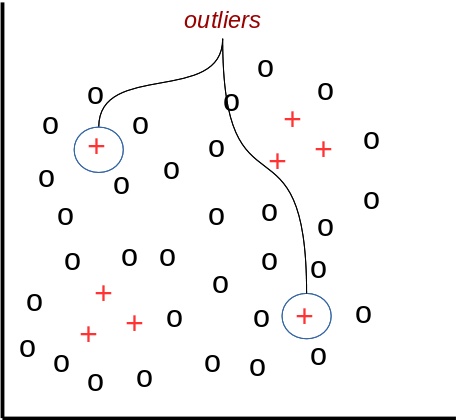
\includegraphics[width=\textwidth]{SMOTE-problem-outliers}
		\caption{}
		\label{fig:smote-outliers}
	\end{subfigure}
	\begin{subfigure}[b]{0.5\textwidth}
		\centering
		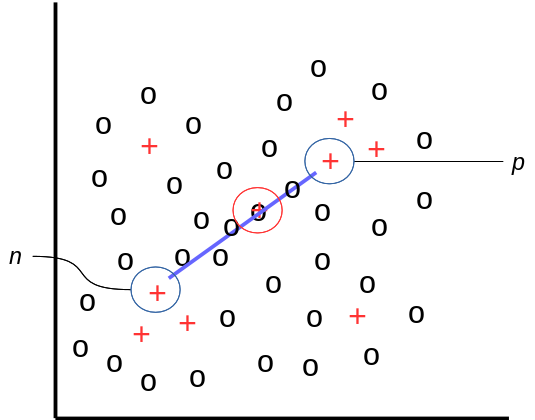
\includegraphics[width=\textwidth]{SMOTE-problem-overlapping}
		\caption{}
		\label{fig:smote-overlapping}
	\end{subfigure}
	\caption{
	Kelemahan pada metode SMOTE:
(a) \textit{Outliers} pada kelas minoritas tidak diperhitungkan pada metode SMOTE.
(b) Pembuatan sampel sintetis yang baru berada di wilayah kelas mayoritas yang tumpang-tindih dengan sampel kelas mayoritas.
	}
	\label{fig:smote-problems}
\end{figure}

Kelemahan lain dari SMOTE yaitu permasalahan \textit{overgeneralization} yang begitu saja menggeneralisasi wilayah dari kelas minoritas.
SMOTE tidak mempertimbangkan distribusi dari sampel pada kelas mayoritas, atau adanya \textit{outliers}.

Untuk mengatasi permasalahan di atas, Maciejewski dkk. memperkenalkan ekstensi dari metode SMOTE bernama \textit{Local-neighbourhood SMOTE} atau disingkat LN-SMOTE \cite{maciejewski2011local} yang menggunakan modifikasi dari pendekatan \textit{Safe-Level SMOTE} \cite{bunkhumpornpat2009safe}.
Pada metode \textit{Safe-level SMOTE} keberadaan sampel mayoritas diperhitungkan sebelum membuat sampel sintetis dengan menghitung sebuah koefisien khusus yang disebut \textit{safe level}.
Untuk setiap sampel dari kelas minoritas, dihitung jumlah sampel kelas minoritas di antara \textit{k-nearest-neighbors}-nya.
Jika nilainya sama atau mendekati 0, sampel tersebut dianggap sebagai \textit{noise}.
Jika nilainya mendekati \textit{k}, maka sampel tersebut bisa dikatakan berada di wilayah aman dari kelas minoritas.
Gagasan utamanya adalah membuat sampel sintetis yang dekat dengan wilayah aman.

Lebih rincinya, misalkan \textit{p} adalah sampel dari kelas minoritas yang akan menjadi calon untuk \textit{over-sampling}, maka sampel \textit{k} terdekat yang termasuk pada kelas minoritas \textit{P} ditentukan.
Seperti pada SMOTE, setidaknya satu dari tetangga tersebut dipilih, sebutlah dengan \textit{n}.
Untuk kedua sampel, \textit{p} dan \textit{n}, sampel \textit{k} terdekatnya untuk keseluruhan data pelatihan \textit{S} dihitung \textit{safe level}-nya dengan notasi \textit{sl(p)} dan \textit{sl(n)}.
Dari pengetahuan tersebut, koefisien rasio \textit{safe-level} ditentukan dengan \textit{sl-ratio = sl(p) / sl(n)}.
Langkah selanjutnya ditentukan berdasarkan 5 kasus berikut:
\begin{enumerate}
	\item \label{case:safe-1} Jika \textit{sl(p) = 0} dan \textit{sl(n) = 0}, sampel \textit{p} dan \textit{n} dianggap sebagai \textit{noise outliers}, dan tidak ada sampel sintetis yang dibuat.
	\item Jika \textit{sl(p) > 0} dan \textit{sl(n) = 0}, maka \textit{n} adalah \textit{noise}.
Sampel sintetis akan dibuat jauh dari \textit{n} dengan menduplikasi \textit{p}.
	\item Jika \textit{sl-ratio = 1}, maka \textit{p} dan \textit{n} memiliki tetangga yang sama dan sampel sintetis yang baru akan dibuat diantara garis yang menghubungkan mereka dengan cara yang sama seperti pada SMOTE.
	\item Jika \textit{sl-ratio > 1}, maka \textit{p} berada di wilayah aman minoritas daripada \textit{n} dan sampel sintetis yang baru akan dibuat dekat dengan \textit{p}, dengan parameter acak pada SMOTE akan memiliki rentang \textit{[0, 1 / sl-ratio]}.
	\item Jika \textit{sl-ratio < 1}, maka \textit{n} berada di wilayah aman minoritas daripada \textit{p} dan sampel sintetis yang baru akan dibuat dekat dengan \textit{n}, yaitu parameter acak pada SMOTE akan memiliki rentang \textit{[1 - sl-ratio, 1]}.
\end{enumerate}

Strategi \textit{safe-level SMOTE} bermasalah khususnya pada distribusi kelas yang bias yang mana kelas minoritas menyebar sehingga terdiri dari beberapa sub-wilayah dengan kardinalitas yang kecil.
Situasi ini mengacu pada permasalahan yang disebut \textit{small disjuncts} yang diakui sebagai sumber kesulitan yang paling penting bagi pembelajaran klasifikasi untuk ketimpangan data \cite{jo2004class}. 
Pada kasus seperti ini pembuatan sampel sintetis dengan \textit{Safe-level SMOTE} bisa menyebabkan terjadinya tumpang-tindih antara kelas.

Sebagai contohnya, misalkan dua kelompok dari kelas minoritas terpisah dikelilingi oleh sampel dari kelas mayoritas.
Katakanlah, jarak antara kedua kelompok minoritas tersebut cukup jauh, satu kelompok berada di bawah dan kelompok lainnya di atas.
Misalkan calon dari sebuah sampel berada di kelompok yang dibawah.
Jika parameter \textit{k} dari fungsi lebih besar dari jumlah sampel kelas minoritas di dalam kelompok tersebut, maka tetangga dari kelas minoritas selanjutnya akan menjadi sampel dari kelompok yang lain.
Jika rasio \textit{safe-level} dari sampel kedua kelompok sama, sampel sintetis yang baru bisa dibuat diantara garis yang menggabungkan sampel-sampel dari kedua kelompok tersebut.
Dengan kata lain, sampel sintetis yang baru bisa berada di wilayah yang dihuni oleh kelas mayoritas.
Makanya, strategi ini masih memungkinkan terjadinya tumpang-tindih antara kelas.

Situasi tidak diinginkan seperti di atas disebabkan karena teknik SMOTE mencari \textit{k-nearest-neighbors} yang dimiliki oleh kelas minoritas saja.
Jika calon sampel tidak berada di wilayah yang padat dengan kelas minoritas, maka beberapa tetangganya bisa saja cukup jauh dan juga sampel dari kelas mayoritas mengelilingi calon sampel tersebut.
LN-SMOTE mengatasi masalah tumpang tindih ini dengan lebih mempertimbangkan \textit{local neighbourhood} dari calon sampel minoritas yang mungkin bisa memberikan perkiraan dari keberadaan sampel kelas mayoritas.
Jadi, pencarian sampel yang terlalu jauh sebaiknya dihindarkan.

Misalnya, jika calon sampel \textit{p} diidentifikasi berada di \textit{k-nearest-neighbors} dari \textit{n}, ia tidak langsung dihitung dengan \textit{sl(n)} tapi dicari tetangga dari \textit{k + 1} selanjutnya.
Modifikasi lain terhadap \textit{safe-level SMOTE} yaitu membatasi rentang interval dimana sampel baru secara acak ditempatkan.
Jadi, pada beberapa kasus dari \textit{safe-level}, LN-SMOTE tidak menentukan batas kanan dari interval dengan 1 tapi sebagai ambang batas $\tau < 1$.
Ambang batas tersebut tidak baku tapi ditentukan secara dinamis bergantung kepada \textit{safe-level} dari sampel mayoritas.
Jika \textit{sl(n)} relatif rendah, artinya \textit{n} dikelilingi oleh banyak sampel dari kelas mayoritas, jadi sampel baru seharusnya ditempatkan lebih dekat ke \textit{p}.
Jika \textit{n} dikelilingi oleh sejumlah sampel minoritas yang seimbang, sehingga nilai \textit{sl(n)} tinggi, sampel yang baru bisa berada di dekat \textit{n}.
Hal ini supaya bisa mengontrol tingkat ekspansi dari kelas minoritas dengan cara dinamis, memperhitungkan distribusi lokal dari sampel-sampel.
